%pictures and spectra
%tables and graphs
%statements of the result


\section{Results}
\label{sec:Results}

In the following the measurement results are going to be presented. 
Therefore some characterizations of the used lightsources are done, as well of other light sources, in order to understand their features as well as the impact of external noise.

\subsection{LED emission spectra}
\label{sec:LED}

\begin{wrapfigure}{l}{\linewidth}
    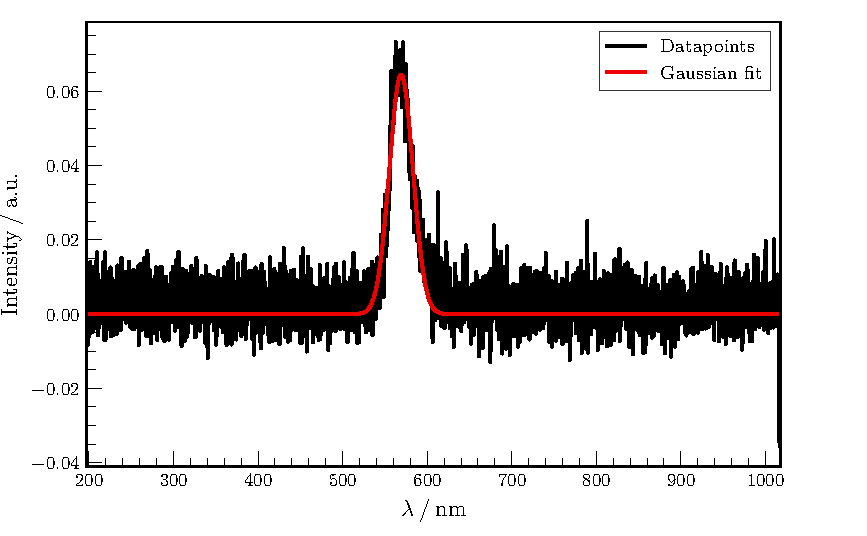
\includegraphics[width=0.5\textwidth]{plots/LED-Green.pdf}
    \caption{Spectral measurement of a green LED lightsourse. A Gaussian fit is implemented.}
    \label{fig:LEDG}
\end{wrapfigure}
\begin{wrapfigure}{r}{\linewidth}
    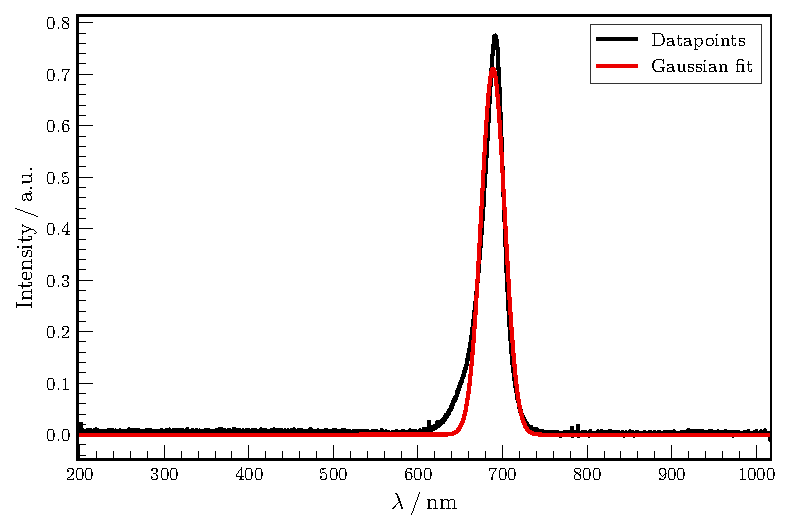
\includegraphics[width=0.5\textwidth]{plots/LED-Red.pdf}
    \caption{Spectral measurement of a red LED lightsourse. A Gaussian fit is implemented.}
    \label{fig:LEDR}
\end{wrapfigure}
\begin{wrapfigure}{r}{\linewidth}
    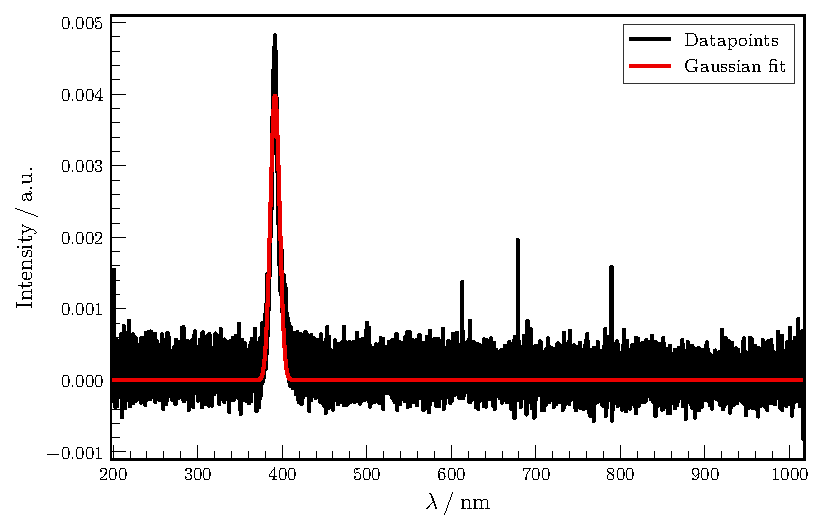
\includegraphics[width=0.5\textwidth]{plots/LED-UV.pdf}
    \caption{Spectral measurement of a UV LED lightsourse. A Gaussian fit is implemented.}
    \label{fig:LEDUV}
\end{wrapfigure}
    

In figure \ref{fig:LEDG},\ref{fig:LEDR},\ref{fig:LEDUV} there are the spectra of a green, red and UV-LED, where a gaussian fit of the form 
\begin{equation}
    f(x,a,b,c) = a \times \exp{-\frac{(x-b^^2)}{2 c^^2}}
\end{equation}
has been introduced. Clearly a $\lambda_\text{peak}$ 
\begin{align*}
    \lambda_\text{peak,green} &= \SI{569.2 \pm 0.2}{\nano\meter} \\
    \lambda_\text{peak,red} &= \SI{688.68 \pm 0.05}{\nano\meter} \\
    \lambda_\text{peak,UV} &= \SI{391.5 \pm 0.1}{\nano\meter} \\
\end{align*}
can be found.
391.4587161187917 \pm 0.09290554731308